\documentclass[a4paper,12pt]{article}
\usepackage[UTF8]{ctex}
\usepackage[text={15.5cm,29cm},left=3.4cm,top=1.2cm]{geometry}
\usepackage{wallpaper,xcolor,multicol}
\pagestyle{empty}\newcommand\mytype[1]{{\fangsong#1}}
\newlength\lengtha
\begin{document}
\ 
\ThisULCornerWallPaper{1}{cover1.jpg}
\newpage
\ThisULCornerWallPaper{1}{cover2.jpg}
\newcommand\mycolora[1]{\textcolor[rgb]{1.00,0.00,0.00}{#1}}\newcommand\mycolorb[1]{\textcolor[rgb]{0.80,0.00,0.55}{#1}}
\newcommand\mycolorc[1]{\textcolor[rgb]{0.05,0.67,0}{#1}}\newcommand\mycolord[1]{\textcolor[rgb]{0.35,0.35,1.00}{#1}}
\newcommand\mytypea[1]{{\kaishu#1}}
 \vspace*{1cm} \centerline{\LARGE \fangsong 自荐书}\vspace*{.5cm} \noindent 尊
敬的领导:\vspace{1ex}

您好!感谢您能在百忙之中审阅我的简历。

\vspace{1ex}我叫王崇宁,来自河南商丘。是西南大学数学与统计学院~2015~届的免费
师范生。谨向贵校自荐,谋取数学教师一职,希望允予考察。

\newcommand\you{\vspace{1ex}\hspace{2.7em}$\textcolor[rgb]{0.00,0.00,1.00}{\triangleright}$}\you\mytypea{一个适合数学的大脑}

大学期间专业课一直名列前茅,除个别科目外,均在~94~分以上,三年来专业成绩
\mycolora{排名第~2}(本专业~280~人),并最终于大三学年荣获\mycolora{国家奖学
金}($T\!O\!P\,4$)。先后获得全国大学生数学建模\mycolorb{重庆市一等奖},
美国数学建模\mycolorb{国际二等奖},一直是队伍里的主力。参加全国大学生数学竞
赛,获得\mycolorb{重庆赛区一等奖}。

解题能力强,有教授数学竞赛的能力和意向。

\you\mytypea{良好的表达能力}

讲话幽默风趣,在讲台上发言总能博得笑声。嗓门很大,普通话良好,普通话测试水平
为一级乙等。大三下学期教育实习期间,表现优异,获得\mycolora{优秀实习生}的称号
(前~5\%),之后在学院组织的\mycolora{讲课比赛}中获得“二等奖”(前~20\%)。

\you\mytypea{一颗注重班级管理的心}

大学~4~年\mycolorb{一直是班委},前两年任学习委员,后两年任团支书兼学习委员。
在全校性选修课的~4~门上任班长,对班级管理经验丰富。经常阅读心理学以及班级管理
方面的书籍,教学技能与管理能力一同进步。班主任对班级成绩起到至关重要的作用,
而我有担任\mycolorb{班主任}的能力和强烈意向。

\you\mytypea{一双有前瞻性的眼睛}

多媒体教学的日益普遍,本人已经拥有熟练的计算机操作技能。获得计算级
\mycolorb{~C语言}二级证书,会编写程序。熟练运用\mycolorb{几何画板}软件,学习
时间~40~小时以上。会用\mycolorb{最强符号数学软件}~Mathematica~,用以解决数学
问题,得心应手。熟练进行屏幕录制,个人录制教学视频。

\par\vspace{2ex}

我非常渴望能够成为贵校的一员, 这将是我一生的荣誉。最后,衷心祝愿贵校事业发
达、蒸蒸日上!

\vspace{1ex}此致\\ 敬礼!\\
\hspace*{\fill} 自荐人: 王崇宁

\newpage\ThisULCornerWallPaper{1}{cover3.jpg}
\ThisULCornerWallPaper{.2}{lu} \ThisLRCornerWallPaper{.2}{rd} \vspace*{0cm}
\begin{multicols}{3}[][1.2in]
 \newcommand\boxa[1]{\raisebox{-22pt}{\hspace{-9pt}#1}}
  \noindent{\LARGE\fangsong 个\boxa{人\boxa{简\boxa{历}}}}
   \par\columnbreak\noindent
    \hspace*{-1em}\textbf{\songti 王崇宁}\\
    \hspace*{-1em}西南大学\ 数学与统计学院\\
    \hspace*{-1em}数学与应用数学(免师)\\
    \hspace*{-1em}男\quad 汉族\quad 中共党员\quad21~岁\\
    \hspace*{-1em}籍贯:河南商丘\\
  \columnbreak\fboxrule=1.2pt\fboxsep=0pt
   \hspace{\fill}\fcolorbox{gray}{white}{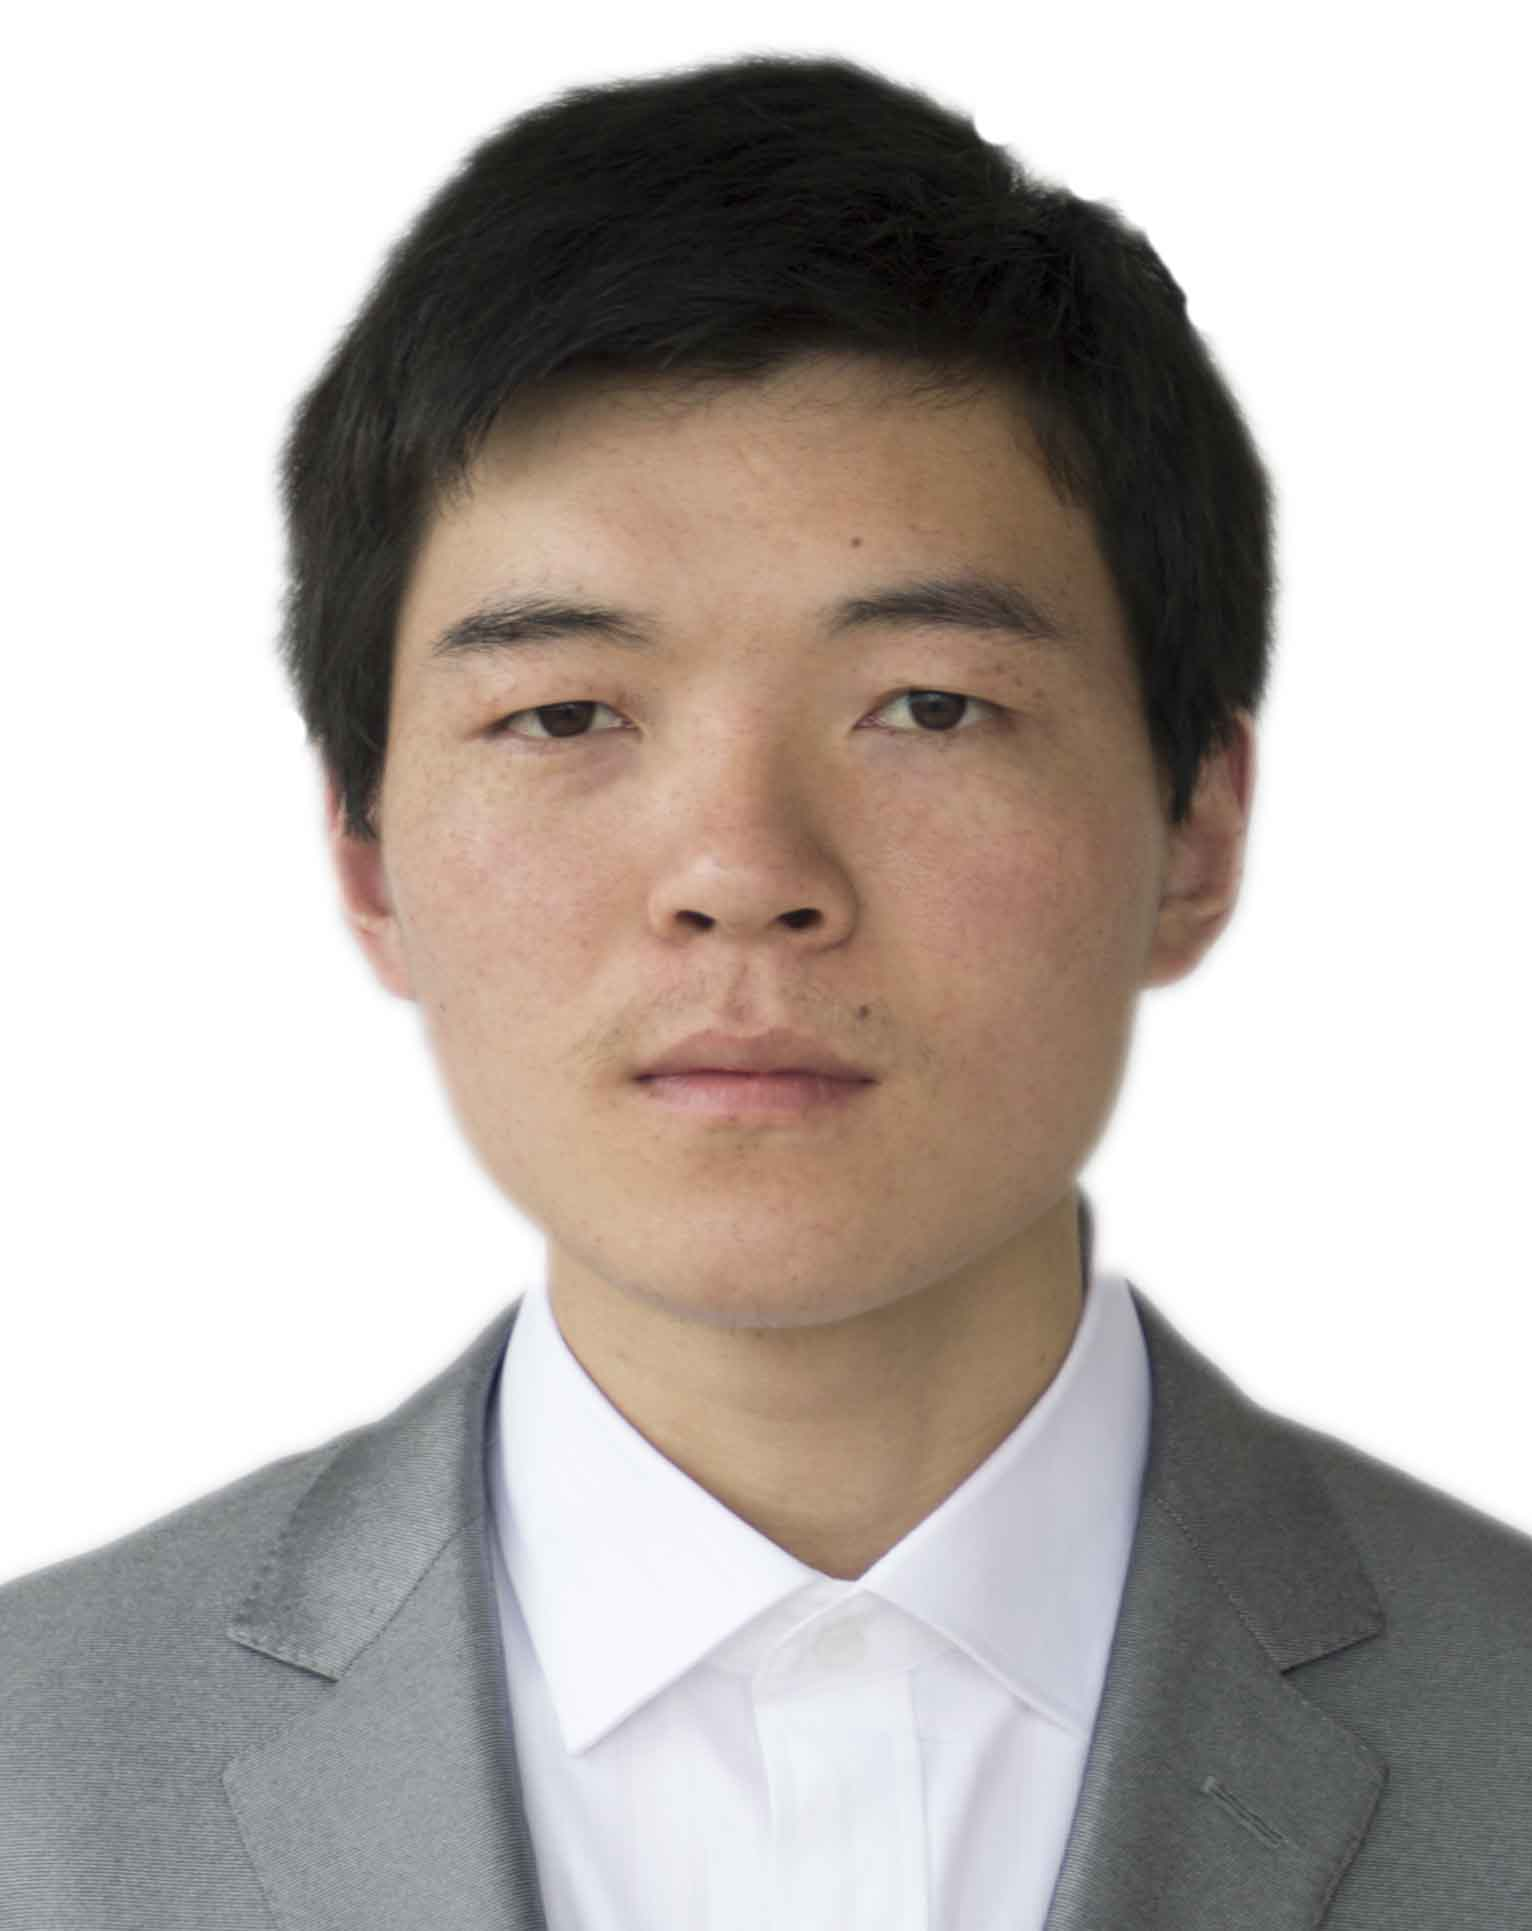
\includegraphics[height=1.4in]{wangchning.jpg}}
\end{multicols}

\newcommand\jobintension[1]{\par\addvspace{-1ex}\hrule\addvspace{2pt}\noindent\raisebox{5pt}{\kaishu{#1}}\songti\quad \settowidth\lengtha{\kaishu{#1}\ \quad}}
 \vspace{2ex} \jobintension{求职意向}中学数学教师\vspace*{3ex}
  \jobintension{教育背景}
西南大学本科,将于~2015~年~6~月获得学士学位                     \hfill    专业排名\textcolor[rgb]{1.00,0.00,0.00}{第~2}\\
\hspace*{\lengtha}2014.3-2014.7~在西南大学附属中学实习        \hfill 获得\textcolor[rgb]{1.00,0.00,0.00}{优秀实习生}\\
\jobintension{获奖情况}
\textcolor[rgb]{1.00,0.00,0.00}{国家奖学金}                    \hfill 2014.09\\
\hspace*{\lengtha}西南大学二等奖学金                            \hfill 2013.12\\
\hspace*{\lengtha}美国\mycolorb{数学建模}国际二等奖              \hfill 2014.04\\
\hspace*{\lengtha}全国大学生\mycolorb{数学建模}重庆市一等奖       \hfill 2013.10\\
\hspace*{\lengtha}全国大学生\mycolorb{数学竞赛}重庆赛区一等奖      \hfill 2013.11\\
\hspace*{\lengtha}学院实习汇报\textcolor[rgb]{1,0,0}{讲课比赛二等奖}\hfill 2014.10\\
\hspace*{\lengtha}西南大学优秀实习生                                 \hfill 2014.10\\
\hspace*{\lengtha}西南大学\mycolora{三好学生}                         \hfill 2013.12\\
\hspace*{\lengtha}西南大学科技创新先进个人                             \hfill 2014.09\\
\hspace*{\lengtha}西南大学体育风尚先进个人                              \hfill 2012.12\\
\hspace*{\lengtha}院级运动会1500米第二名                                 \hfill 2012.12\\
\jobintension{任职情况}\ 班级负责人       \hfill 2014.9至今\\
\hspace*{\lengtha}班级\mycolorb{团支部书记}\hfill 2013-2014\\
\hspace*{\lengtha}班级学习委员              \hfill 2012-2013\\
\hspace*{\lengtha}班级学习委员               \hfill 2011-2012\\
\jobintension{职业技能}
普通话(一级乙等:92.1分)                     \hfill 2012.11\\
\hspace*{\lengtha}C语言二级(合格)             \hfill 2013.03\\
\jobintension{兴趣爱好}
长于逻辑思维, 喜欢趣味数学和竞赛数学\\
\hspace*{\lengtha}喜欢心理学, 乐于班级管理\\
\hspace*{\lengtha}爱好跑步:\mycolord{运动使人聪明}. 拉二胡:\mycolord{音乐自含深情}. 摄影:\mycolord{图远胜于文字}\\
\hspace*{\lengtha}重视计算机在教学上的应用, 熟用mathematica, 几何画板等数学软件 \\
\jobintension{教学理念}
教育事业值得我\mycolorc{奉献一生}。\\
\hspace*{\lengtha}一个班级好坏的决定因素在于\mycolorc{班主任}。\\
\par\addvspace{-1ex}\hrule
\begin{center}\vspace*{2ex}手机:13650565628\quad 邮箱:wangchning@163.com\\
\end{center}
%%%证书
\newpage\fboxrule=1.2pt\fboxsep=0pt\setlength\lengtha{94mm}
\newcommand\picturea[1]{\hspace*{1cm}\fcolorbox{gray}{white}{\includegraphics[width=1.5\lengtha,height=\lengtha]{#1}}\\\vspace*{-2pt}}
\begin{center}
\ThisULCornerWallPaper{1}{cover3.jpg}\vspace*{-1cm}\picturea{wcn1}\picturea{wcn2}\picturea{wcn3}\newpage
\ThisULCornerWallPaper{1}{cover3.jpg}\vspace*{-1cm}\picturea{wcn9}\picturea{wcn10}\picturea{wcn18}\newpage
\ThisULCornerWallPaper{1}{cover3.jpg}\vspace*{-1cm}\picturea{wcn4}\picturea{wcn5}\picturea{wcn6}\newpage
\ThisULCornerWallPaper{1}{cover3.jpg}\vspace*{-1cm}\picturea{wcn13}\picturea{wcn14}\picturea{wcn15}\newpage
\end{center}
\ \ThisULCornerWallPaper{1}{cjd.jpg}
\end{document}
